\documentclass[../diplomski_rad.tex]{subfiles}

\begin{document}

\sloppy

\justifying

\section{Bioimpedancija}

Bioimpedancija predstavlja impedanciju koji se javlja kada kroz biološka tkiva teče električna struja \cite{Bera2014}.
Ovisna je o frekvenciji te se može prikazati formulom:
\begin{equation}
    \label{jed:cpe}
    Z(f) = R_{e}(f) + jI_{m}(f) = |Z(f)|\angle\theta(f) 
\end{equation}
gdje je
\begin{equation}
    \label{jed:cpe}
    |Z(f)| = \sqrt{R_{e}^{2} + I_{m}^{2}}
\end{equation} 
\begin{equation}
    \label{jed:cpe}
    \theta(f) = arctg(\frac{I_{m}}{R_{e}})
\end{equation} 

\begin{figure}[htb]
    \centering
    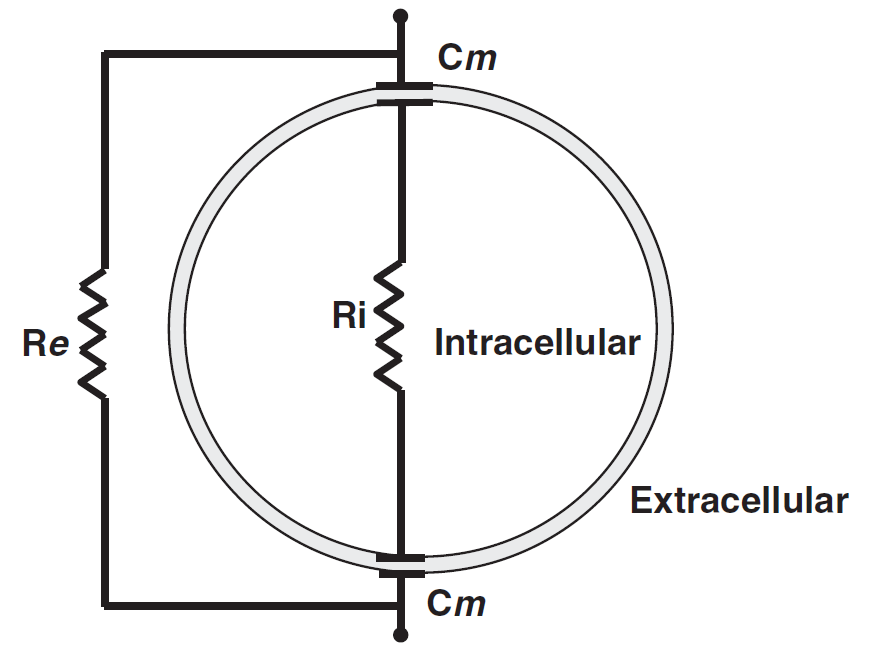
\includegraphics[width=0.6\textwidth]{Figures/stanica.png} 
    \caption{Električni model stanice \cite{Lukaski2013}}
    \label{slk:stanica}
\end{figure}
Za razumijevanje protoka električne struje kroz ljudsko tijelo, potrebno je detaljno prikazati električni model stanice.
Ljudska stanica može se modelirati ekvivalentnom električnom RC mrežom \cite{Lukaski2013}, 
kao što je prikazano na slici \ref{slk:stanica}. 
$R_{e}$ predstavlja otpor ekstracelularne tekućine dok $R_{i}$ predstavlja otpor intracelularne tekućine.
Stanična membrana zbog svojih kapacitivnih svojstava, prikazanih kapacitetom $C_{m}$, 
propušta struju visokih frekvencija, dok struje niskih frekvencija blokira. 
Zbog toga postoji razlika u mjerenoj impedanciji u ovisnosti o frekvenciji uzbudne struje. 
Na niskim frekvencijama struja samo vidi otpor $R_{e}$ ekstracelularne tekućine, dok se na visokim frekvencijama dodaje i otpor 
$R_{i}$ intracelularne tekućine čime ukupna impedancija pada \cite{Bera2014}.

Matematički model kojim se najčešće modelira bioimpedancija ljudskog tijela naziva se Cole-Cole model.  
Cole-Cole model opisuje impedanciju tijela kao funkciju frekvencije zbog čega ga koristimo pri analizi sastava ljudskog tijela \cite{Freeborn2021}.
\begin{figure}[htb]
    \centering
    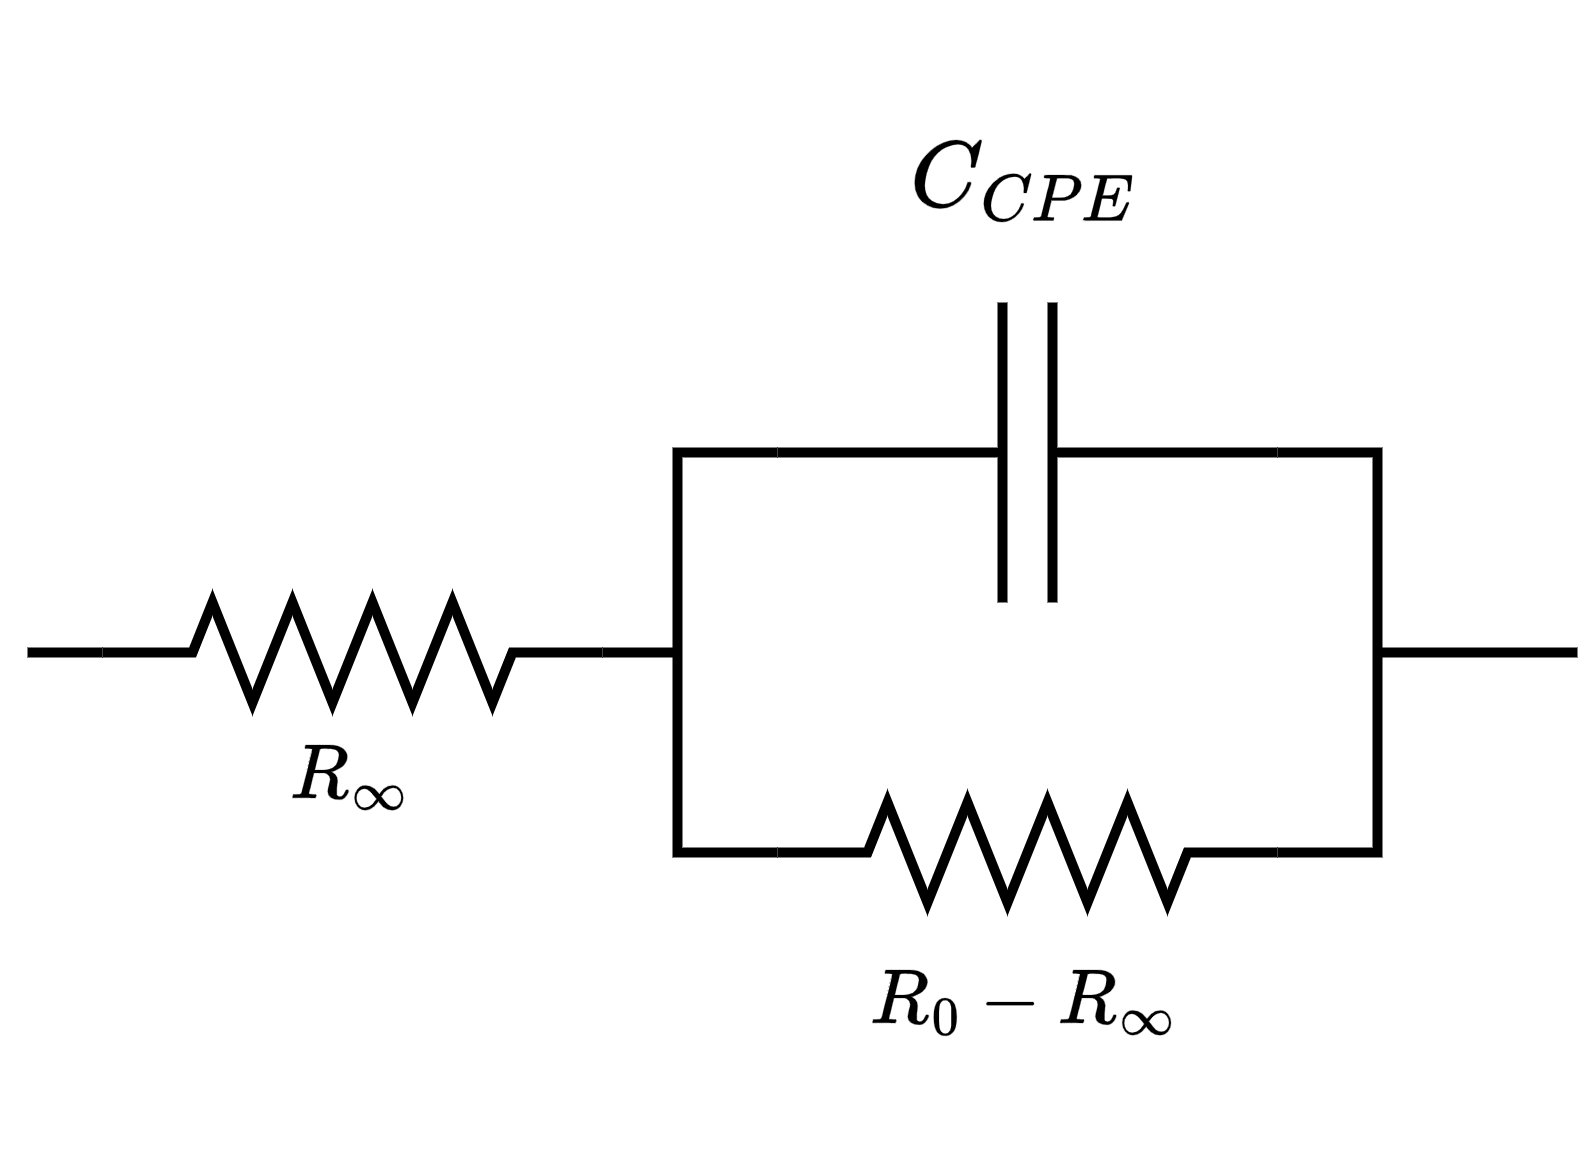
\includegraphics[width=0.6\textwidth]{Figures/cole_model.png} 
    \caption{Cole-Cole model bioimpedancije}
    \label{slk:cole_model}
\end{figure}
$R_{\infty}$ predstavlja otpor tkiva na beskonačnoj frekvenciji dok $R_{0}$ predstavlja otpor na nultoj frekvenciji. 
Razlika otpora $R_{0}-R_{\infty}$ predstavlja dodatni otpor struji na niskim frekvencijama zbog nepropusnosti stanične membrane. 
$C_{CPE}$ je element s konstantnom fazom koji modelira kapacitivnost stanične membrane 
te predstavlja neidealan kondenzator. Njegova impedancija iznosi: 
\begin{equation}
    \label{jed:cpe}
    Z_{CPE}(\omega) = \frac{1}{(j\omega)^{\alpha}C}
\end{equation} 
gdje je C kapacitet, a $\alpha$ njegov red. Kada je $\alpha = 0$ element s konstantnom fazom predstavlja idealan otpornik, 
dok sa $\alpha = 1$ predstavlja idealan kondenzator. 
Tipične vrijednosti parametra $\alpha$ za biološka tkiva su u intervalu 0.5 $< \alpha <$ 1 \cite{Freeborn2021}.
Ako uvedemo karakterističnu vremensku konstantu $\tau$ kao
\begin{equation}
    \label{jed:time_const}
    \tau = [(R_{0}-R_{\infty})C]^{1/\alpha}
\end{equation}
dobivamo originalnu jednadžbu Cole-Cole modela: 
\begin{equation}
    \label{jed:cole}
    Z(\omega) = R_{\infty}+\frac{R_{0}-R_{\infty}}{1+(j\omega\tau)^{\alpha}} 
\end{equation} 
Iz jednadžbe \ref{jed:cole} vidljivo je kako su parametri Cole-Cole modela bioimpedancije 
$R_{\infty}$, $R_{0}$, $\alpha$ i $\tau$. 
Svojstva tkiva opisuju se pomoću navedenih parametra, a postupak kojim se do njih dolazi opisan je u daljnjem tekstu.

Rezultati mjerenja bioimpedancije na različitim frekvencijama mogu se aproksimirati polukružnicom,  
što je prikazano na slici \ref{slk:cole_graf}. 
Graf prikazuje omjer negativne reaktancije i otpora tkiva na svim frekvencijama, 
od $f=0$ do $f=\infty$. Frekvencija raste s desna na lijevo. 
\begin{figure}[htb]
    \centering
    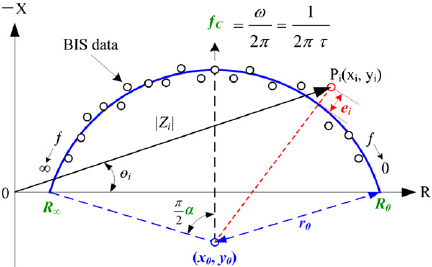
\includegraphics[width=0.7\textwidth]{Figures/cole_plot.png} 
    \caption{Graf bioimpedancije Cole-Cole modela \cite{Yang_2013}}
    \label{slk:cole_graf}
\end{figure}
Iz opisanog grafa moguće je dobiti parametre Cole-Cole modela \cite{Yang_2013}.
$R_{\infty}$ i $R_{0}$ jednostavno se iščitavaju kao presjecišta polukružnice i realne osi.
Vremenska konstanta $\tau$ inverz je karakteristične kružne frekvencije $\omega_{C}$ na kojoj je reaktancija najveća.
Relacija iz koje se izračunava $\tau$ je:
\begin{equation}
    \label{jed:cole}
    f_{C} = \frac{\omega_{C}}{2\pi} = \frac{1}{2\pi\tau} 
\end{equation} 
Parametar $\alpha$ određuje koliko je središte kružnice pomaknuto ispod realne osi. 
Izračunava se iz kuta između karakteristične frekvencije $f_{C}$ i beskonačne frekvencije $f_{\infty}$. 
Ako se taj kut definira kao $\theta$, vrijedi sljedeći izraz:
\begin{equation}
    \label{jed:cole}
    \theta = \frac{\pi}{2}\alpha 
\end{equation} 

\section{Pregled metoda mjerenja bioimpedancije}
Analiza bioimpedancije (engl. \textit{Bioelectrical Impedance Analysis; BIA}) klasificira se u dva pristupa: 
analiza s jednom frekvencijom (engl. \textit{Single frequency BIA; SF-BIA}) 
i analiza s višestrukim frekvencijama (engl. \textit{Multi frequency BIA; MF-BIA}).
Važna metoda je i bioelektrična spektrografija (engl. \textit{Bioelectrical spectroscopy; BIS}) 
koja daje rezultate kroz širok raspon frekvencija. 

SF-BIA je najjednostavnija i najbrža metoda jer koristi samo mjerenje impedancije na jednoj frekvenciji, najčešće 50 kHz. 
Iz izmjerene bioimpedancije matematičkim izračunima dobivaju se ukupna tjelesna voda, mišićna masa i masa masnog tkiva. 
Ova metoda ima najmanju preciznost jer se podatci prikupljaju na samo jednoj frekvenciji uzbudne struje.

MF-BIA koristi nekoliko različitih frekvencija čime se postiže veća točnost i mogućnost procjene dodatnih parametara, 
kao što su količine intracelularne i ekstracelularne vode. To je moguće jer stanična membrana blokira struju na niskim frekvencijama, 
a propušta ju na višim. 

Bioelektrička spektrografija najpreciznija je metoda mjerenja bioimpedancije. 
Mjerenja se obavljaju na širokom rasponu frekvencija, od 1 kHz do 1 MHz.  
Ovom metodom možemo procijeniti otpor na nultoj i beskonačnoj frekvenciji, parametre iz Cole-Cole modela bioimpedancije 
opisane u prethodnom poglavlju. 
Mjerenje BIS metodom zbog većeg broja frekvencija traje duže i matematički izračuni su složeniji, 
ali pruža  detaljniju i precizniju analizu sastava ljudskog tijela.

Postupak mjerenja bioimpedancije svih ranije opisanih metoda je puštanje slabe, 
frekvencijski ovisne izmjenične struje kroz tkivo te mjerenje pada napona \cite{Bera2014}. 
Zatim se impedancija izračunava prema:
\begin{equation}
    \label{jed:prvajednadzba}
    Z\angle\theta = \frac{U\angle\theta_{1}}{I\angle\theta_{2}} 
\end{equation} 

Pri mjerenju bioimpedancije razlikujemo dvožično i četverožično spajanje elektroda. 
Kod dvožičnog mjerenja isti par elektroda služi za pobudnu struju i za mjerenje napona. 
Zbog toga dolazi do pogreške u mjerenju napona uzrokovane padom napona na elektrodama. 
Četverožično mjerenje je preciznije jer se pad napona mjeri izravno na koži i zbog toga će se koristiti u ovom radu \cite{Abasi2022}. 

\begin{figure}[htb]
    \centering
    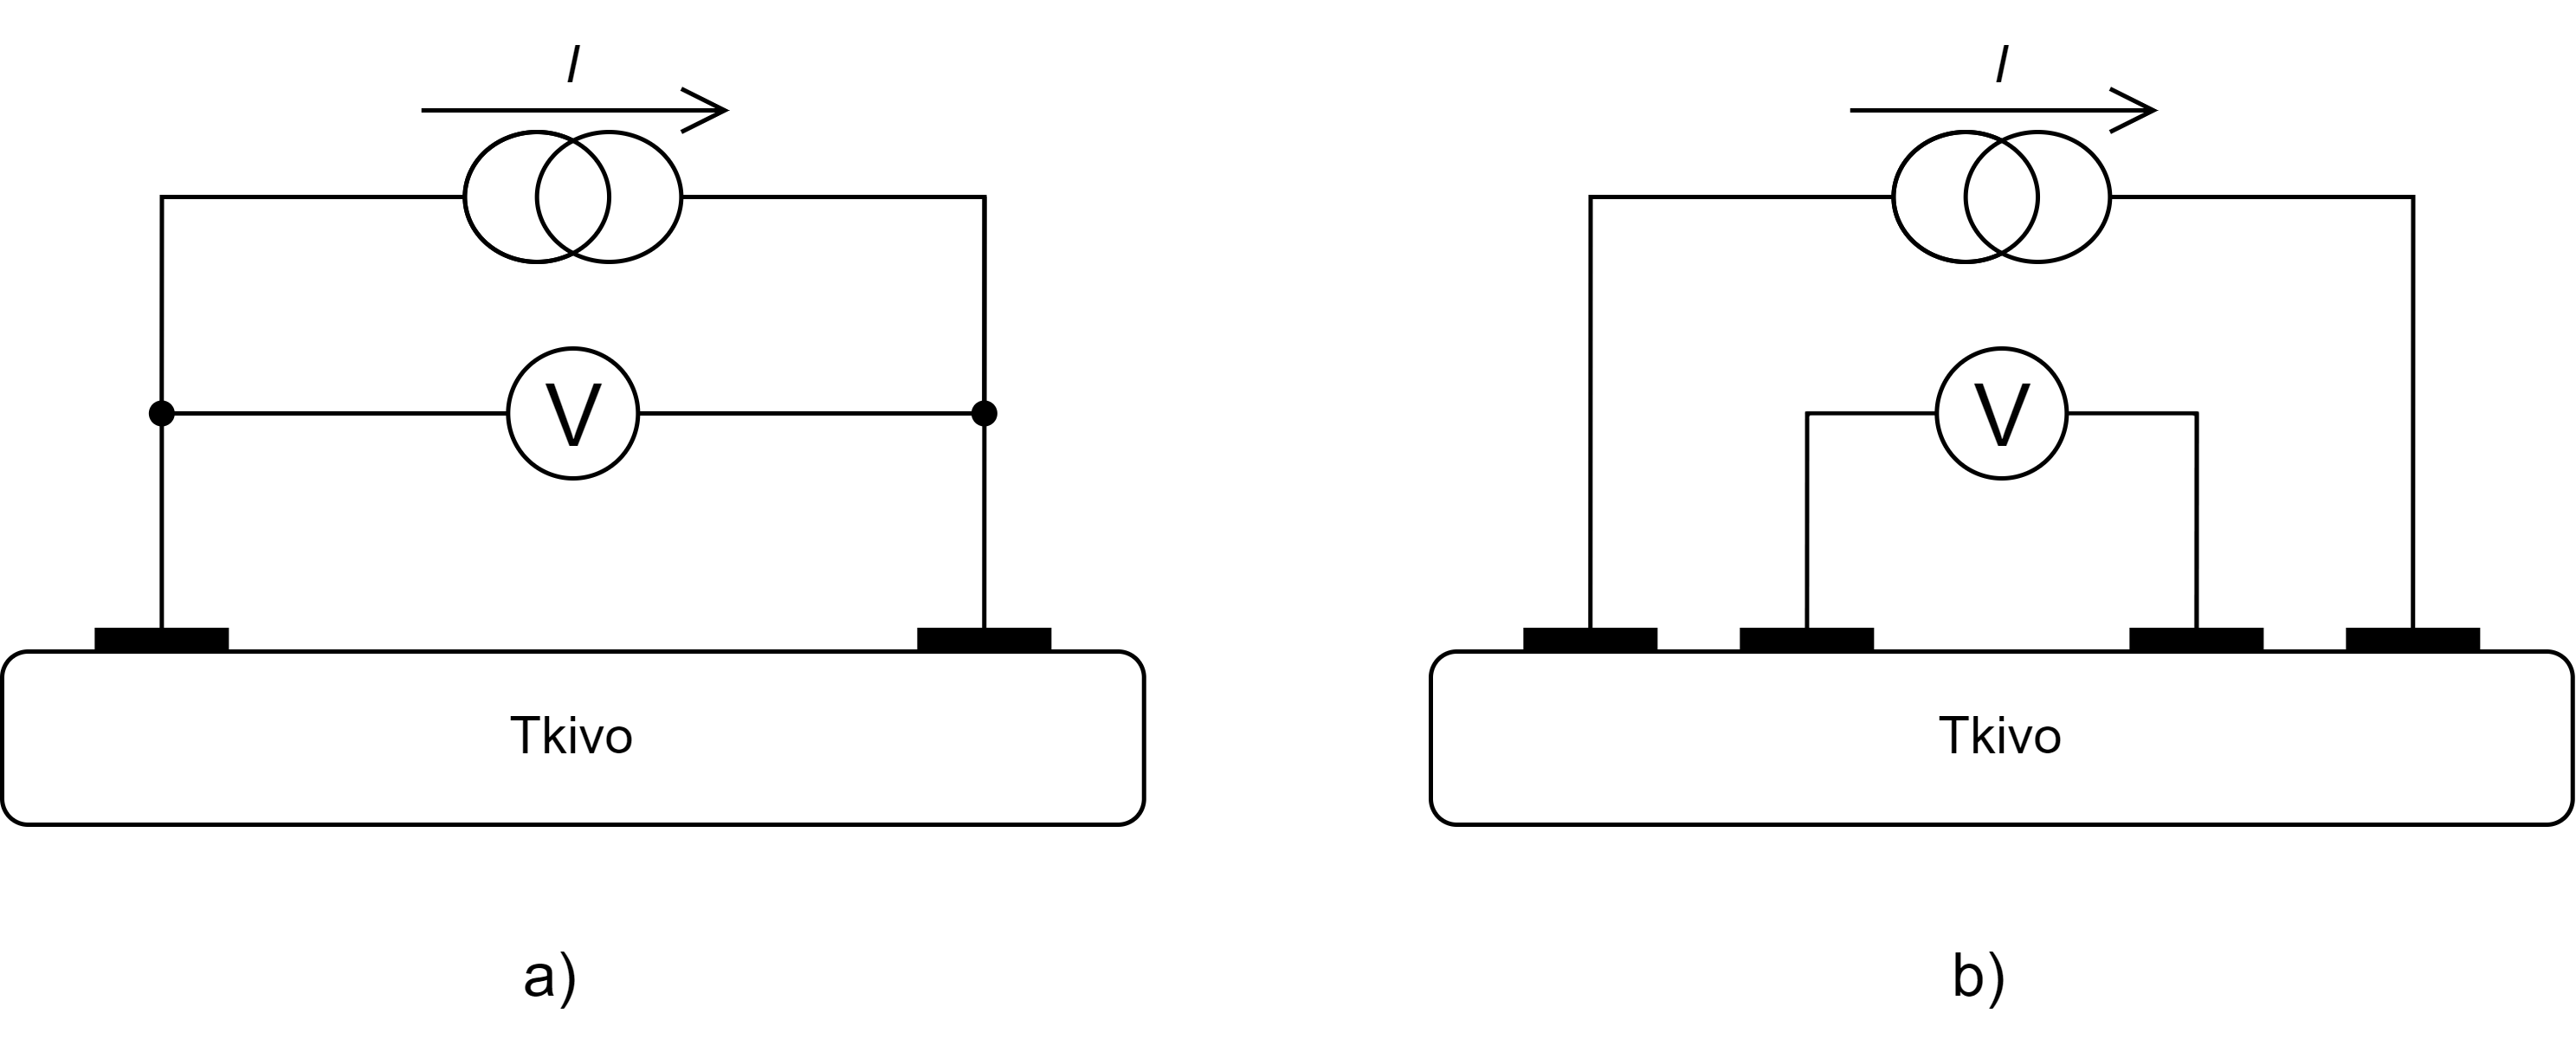
\includegraphics[width=0.8\textwidth]{Figures/dvo_vs_cetverozicno.png} 
    \caption{Dvožično (a) i četverožično (b) mjerenje bioimpedancije}
    \label{slk:cole_model}
\end{figure}

Sve opisane metode predstavljaju jednostavan i neinvazivan postupak mjerenja bioimpedancije. 
Važno je napomenuti kako izmjerena impedancija ovisi o brojim faktorima, kao što su položaj tijela, hidracija, temperatura tijela i drugi 
što treba uzeti u obzir pri obradi rezultata mjerenja.

\newpage

\section{Komercijalno dostupni uređaji za mjerenje bioimpedancije}

Neki od komercijalnih uređaja za mjerenje bioimpedancije prikazani su u tablici \ref{tab:komercijalni_uredaji}.

\begin{table}[H]
\centering
\begin{tblr}{
    width=1\linewidth,
    cells={valign=m,halign=c},
    row{1}={bg=lightgray,font=\bfseries,rowsep=8pt},
    column{1}={2cm},
    column{2}={9cm},
    column{3}={3cm},
    hlines,
    vlines
}
    \hline
    Uređaj & Opis & Autor i godina \\ [0.5ex] 
    \hline\hline
    BIA 101 (Akern) & Uređaj za bioimpedancijsku analizu, koristi se u sportskoj medicini, nutricionizmu i kliničkoj dijagnostici. & Więch, et al. (2022) \cite{Wiech2022} \\
    \hline
    InBody 770 (InBody) & Napredni uređaj za mjerenje bioimpedancije, pruža detaljne analize tjelesnog sastava. Koristi se u kliničkim ustanovama i istraživačkim laboratorijima. & Choi, et al. (2022) \cite{Choi2022}  \\ 
    \hline
    Tanita MC-780U & Uređaj za višefrekvencijsku bioimpedancijsku analizu, koristi se u fitness centrima, bolnicama i za istraživačke svrhe. & Ślązak, et al. (2024) \cite{Slazak2024} \\
    \hline
    ImpediMed SFB7 & Uređaj koji koristi višefrekvencijsku bioimpedancijsku spektroskopiju za procjenu tjelesnog sastava, koristi se u kliničkim istraživanjima. & Freeborn, et al. (2018) \cite{Freeborn2018}  \\
    \hline
    SECA mBCA 515 & Medicinski uređaj za analizu tjelesnog sastava, pruža podatke o masnoj masi, mišićnoj masi i hidrataciji tijela. & Lahav, et al. (2021) \cite{Lahav2021} \\
    \hline
\end{tblr}
\caption{\label{tab:komercijalni_uredaji}Komercijalni uređaji za mjerenje bioimpedancije.}
\end{table}

BIA 101 Anniversary Sport Edition (Akern) je uređaj za bioimpedancijsku analizu koji se koristi u različitim kliničkim 
i istraživačkim okruženjima, posebno u sportskoj medicini, nutricionizmu i kliničkoj dijagnostici \cite{Wiech2022}.  
InBody 770 je napredni uređaj za mjerenje bioimpedancije koji pruža detaljne analize tjelesnog sastava, 
uključujući mišićnu masu, masno tkivo i tjelesnu vodu.  
Koristi se u kliničkim ustanovama i istraživačkim laboratorijima \cite{Choi2022}. 
Tanita MC-780U je uređaj za višefrekvencijsku bioimpedancijsku analizu koji omogućuje precizno mjerenje tjelesnog sastava. 
Ovaj uređaj se često koristi u fitness centrima, bolnicama i za istraživačke svrhe \cite{Slazak2024}. 
ImpediMed SFB7 koristi višefrekvencijsku bioimpedancijsku spektroskopiju za procjenu tjelesnog sastava, 
uključujući tjelesnu vodu, staničnu masu i masno tkivo, te se često koristi u kliničkim istraživanjima \cite{Freeborn2018}. 
SECA mBCA 515 je medicinski uređaj za analizu tjelesnog sastava koji koristi bioimpedancijsku analizu 
kako bi pružio detaljne podatke o masnoj masi, mišićnoj masi i hidrataciji tijela \cite{Lahav2021}. 

Iako su svi ovi uređaji vrlo precizni i korisni u određenim kontekstima, 
njihova glavna ograničenja uključuju ograničenu frekvenciju mjerenja, 
neprilagođenost za kontinuirano praćenje te potrebu za specifičnim uvjetima i postavkama za točna mjerenja. 
Ovo ih čini nepraktičnima za pacijente koji trebaju kontinuirano praćenje, posebno kod srčanih bolesnika 
gdje je kontinuirano mjerenje bitno za pravovremeno otkrivanje promjena u zdravstvenom stanju.

Razvoj nosivog sustava za kontinuirano praćenje bioimpedancije 
temeljenog na MAX30009 je važno zbog ovih ograničenja. 
Srčani bolesnici zahtijevaju stalno praćenje kako bi se na vrijeme otkrile promjene u volumenu tjelesne tekućine, 
što je ključno za pravovremenu medicinsku intervenciju. Kontinuirano praćenje omogućava bolje 
upravljanje stanjem pacijenta i prevenciju ozbiljnijih komplikacija. 
Uređaj temeljen na MAX30009 nudi mogućnost prenosivosti, konstantnog mjerenja i prilagodbe korisnicima, 
čime se osigurava pouzdanost i učinkovitost u stvarnim uvjetima korištenja.

\begin{figure}[htb]
    \centering
    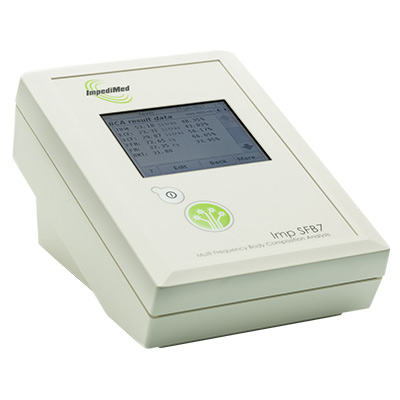
\includegraphics[width=0.45\textwidth]{Figures/sfb7.jpg} 
    \caption{SFB7 ImpediMed uređaj \cite{sfb7}}
    \label{slk:sfb7}
\end{figure}

U kontekstu razvoja nosivog uređaja za mjerenje bioimpedancije, SFB7 ImpediMed 
koristi se kao referentni uređaj za usporedbu i validaciju rezultata \cite{sfb7}. 
SFB7 ImpediMed koristi četverokanalno mjerenje te u jednom mjerenju, koje traje približno jednu sekundu, očitava 256 frekvencija. 
Očitane frekvencije su iz raspona 3 kHz do 1 MHz \cite{sfb7}. 
Koristeći SFB7 ImpediMed kao referencu, omogućava se usporedba performansi i identifikacija 
mogućih poboljšanja ili prilagodbi na novom nosivom uređaju. 

\end{document}